\section{Priority search tree: cont}
\label{sec:range-queries}

This section is a continuation of the last session on Priority Search Trees (PSTs) where we are interested to dive deeper into the analysis of PSTs. Before going into details, we need to recall PST with $P_{ymax}$ as the point with the largest $y-$coordinate and $x_{med}$ as the median $x$-coordinate among points in the input set $S$. A PST can be built up as shown in Figure~\ref{fig:PST1} where $S_{left}$ and $S_{right}$ are obtained as follows:
\begin{align*}
    & S_{left}=\{P \in S\setminus \{p_{ymax}\} \mid P.x \leq x_{med} \}\\
    &  S_{right}=\{P \in S\setminus \{p_{ymax}\} \mid P.x > x_{med} \}
\end{align*}
\begin{figure}[h!]
\begin{center}
  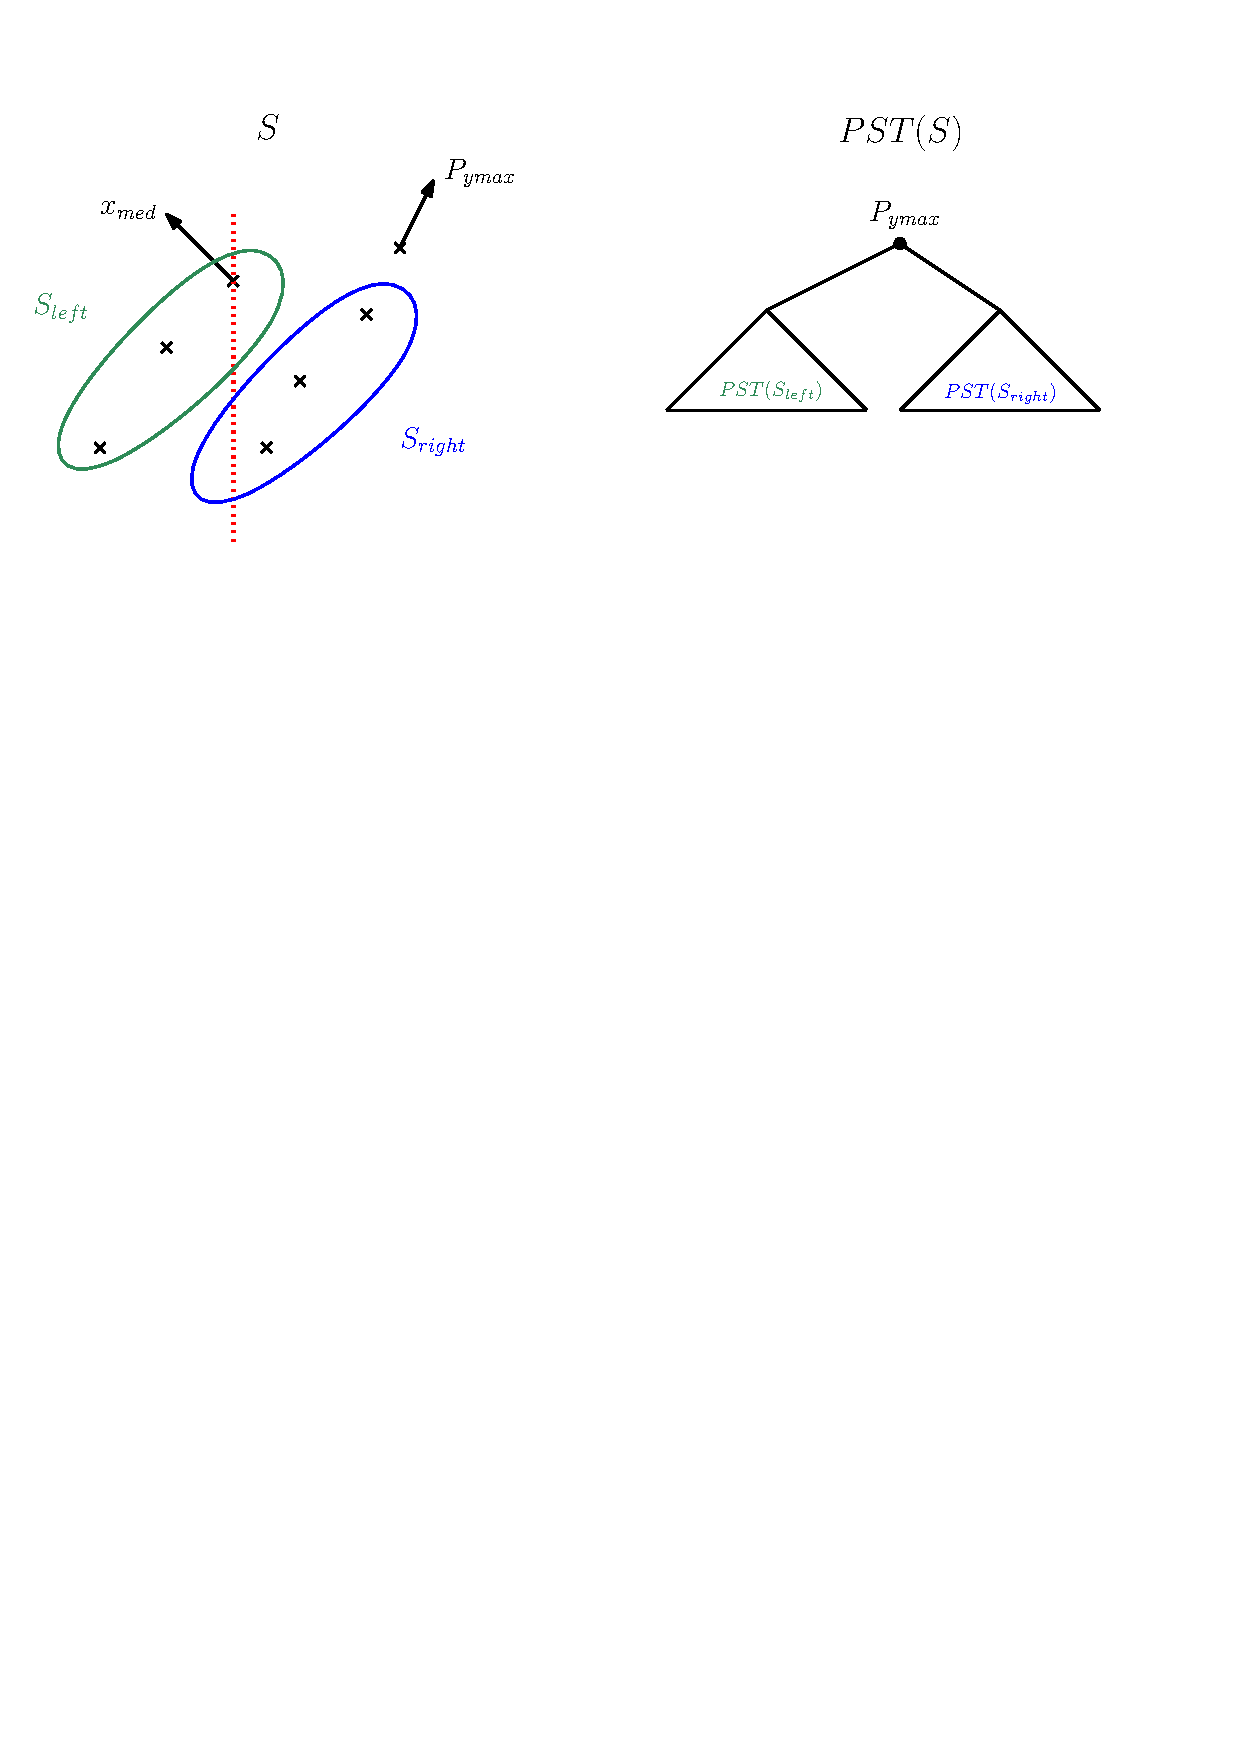
\includegraphics[scale = .5]{ipe/RQ1.pdf}
  \vspace{-0.1in}
  \caption{Building priority search tree.}
  \label{fig:PST1}
\end{center}
\end{figure}

To report all nodes in a subtree rooted at $v$, we can use the following pseudocode:
\begin{algorithm}[H]
\caption{Report a subtree in PST}\label{Report_subtree1}
\begin{algorithmic}[1]
\Function{Report}{$v$}
\If {$v \neq NULL$}
    \State \Call{Output}{$v$}
    \State \Call{Report}{$v.left$}
    \State \Call{Report}{$v.right$}
\EndIf
\EndFunction
\end{algorithmic}
\end{algorithm}

\subsection{Range Query}
Let's consider a range query in one dimensional space where we're asked to report all points greater than or equal to a real number $q_y$. In this case, we can use the following pseudocode to report all nodes above $q_y$ in a subtree rooted at $v$.
\begin{algorithm}[H]
\caption{Report a subtree above $q_y$ in PST}\label{Report_subtree2}
\begin{algorithmic}[1]
\Function{Report}{$v, q_y$}
\If {$v \neq NULL$}
    \If {$v.y \geq q_y$}
        \State \Call{Output}{$v$}
        \State \Call{Report}{$v.left, q_y$}
        \State \Call{Report}{$v.right, q_y$}
    \EndIf
\EndIf
\EndFunction
\end{algorithmic}
\end{algorithm}
The above pseudocode reports all the points above $q_y$ because any path from root $v$ to any node is in a non-decreasing order of $y-$coordinate (otherwise the property of PST doesn't hold). Likewise, the subtree of nodes needs to be reported is either connected and contains the root or it is empty.

The performance of PSTs is summarized in the following theorem.
\begin{theorem}\label{theorem1:RQ}
The total running time to report all points in a query range $[q_y, +\infty]$ in a PST rooted at $v$ is:
\begin{equation*}
    T(v) = c\cdot k_v + c - 1
\end{equation*}
where $k_v$ is the number of reported points and $c \geq 1$.
\end{theorem}

\begin{proof}
We prove the theorem by using the induction.\\
\textit{Induction hypothesis:} For all descendant nodes $u$ of $v$:
\begin{equation*}
    T(u) = c\cdot k_u + c-1
\end{equation*}
where $k_u$ is the total number of nodes above $q_y$ in a PST rooted at $u$.\\

For the base case where there is no point in the query above $q_y$, the theorem is true. Now we show that it's also true for the PST rooted at $v$.
\begin{align*}
    T(v) &= 1 + T(v.left)+ T(v.right)\\
    &= 1 + c\cdot k_{v.left} + c-1 + c\cdot k_{v.right} + c-1 \\
    &= c-1 + c(1+k_{v.left}+k_{v.right})\\
    &= c-1 + c\cdot k_v \qedhere
\end{align*}
\end{proof}

\subsection{3-sided Range Query}

Now, let's look at 2D range query where we aim to find nodes within a 3-sided range (i.e. $[x_L, x_R] \times [y, +\infty]$) as shown in Figure~\ref{fig:PST2}.
\begin{figure}[h!]
\begin{center}
  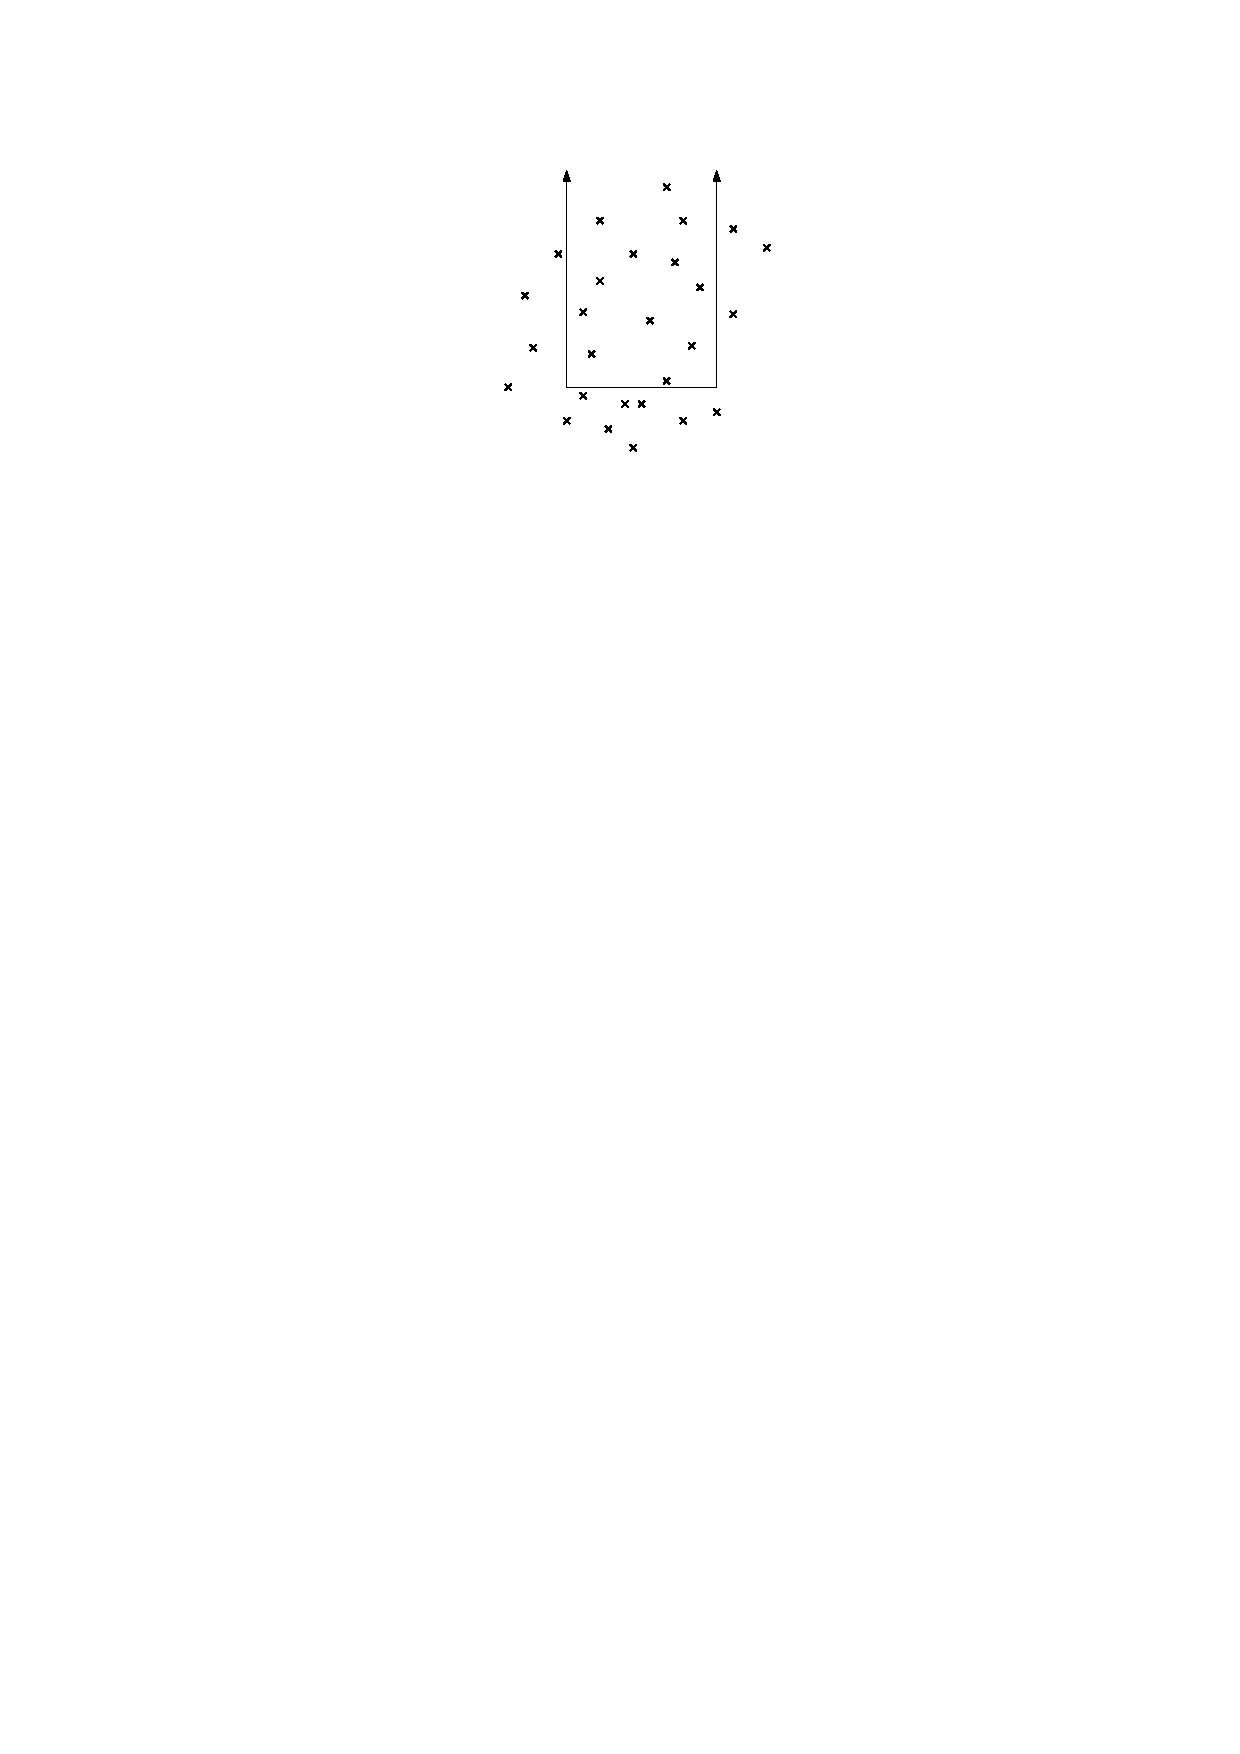
\includegraphics[scale = 1]{ipe/RQ2.pdf}
  \vspace{-0.1in}
  \caption{3-sided Range Query.}
  \label{fig:PST2}
\end{center}
\end{figure}


We follow the subsequent steps to report all nodes corresponding to the specified range:
\begin{itemize}
    \item Find splitting vertex $v_{split}$.
    \item Follow left path down to $x_L$ (left boundary) and report all points in the subtrees hanging from the right.
    \item Follow right path down to $x_R$ (right boundary) and report all points in the subtrees hanging from the left.
\end{itemize}
The pseudocode shown in Algorithm~\ref{3-sided} describes the query algorithm.

\begin{algorithm}[h!]
\caption{3-sided Range Query}
\label{3-sided}
\begin{algorithmic}[1]
\Function{3-sided Query}{$v, [x_L, x_R], y$}
\While{$(v \neq NULL) \textbf{and} (v.x_{med} \leq x_L \ \textbf{or} \ x_R < v.x_{med})$} \Comment{Find the node where paths split}
    \If {$v \in [x_L, x_R] \times [y, +\infty]$}
        \State \Call{Output}{$v$}
    \EndIf
    \If {$v.x_{med} \leq x_L$}
        \State {$v = v.right $}
    \Else
        \State {$v = v.left $}
    \EndIf
\EndWhile
    \State {$v_{split} = v$}
    \State {$v = v.left$}
    \If {$v_{split} \in [x_L, x_R] \times [y, +\infty]$}
        \State \Call{Output}{$v_{split}$}
    \EndIf

\While{$v \neq NULL$}   \Comment{Follow the left path}
    \If {$v \in [x_L, x_R] \times [y, +\infty]$}
        \State \Call{Output}{$v$}
    \EndIf
    \If {$x_L \leq v.x_{med}$}
        \State \Call{Report}{$v.right, y$}
        \State {$v = v.left$}
    \Else
        \State {$v = v.right $}
    \EndIf
\EndWhile
\State {$v = v_{split}.right$}

\While{$v \neq NULL$}   \Comment{Follow the right path}
    \If {$v \in [x_L, x_R] \times [y, +\infty]$}
        \State \Call{Output}{$v$}
    \EndIf
    \If {$v.x_{med} \leq x_R$}
        \State \Call{Report}{$v.left, y$}
        \State {$v = v.right$}
    \Else
        \State {$v = v.left $}
    \EndIf
\EndWhile
\EndFunction
\end{algorithmic}
\end{algorithm}

We start to find the splitting point with $x_L$ and $x_R$ as shown in Figure~\ref{fig:PST3}. All shaded subtrees are those whose $x-$coordinate lies in the specified range. Therefore, we can search those subtrees based on just $y-$coordinate as given in Algorithm~\ref{Report_subtree2}. 

\begin{figure}[h!]
\begin{center}
  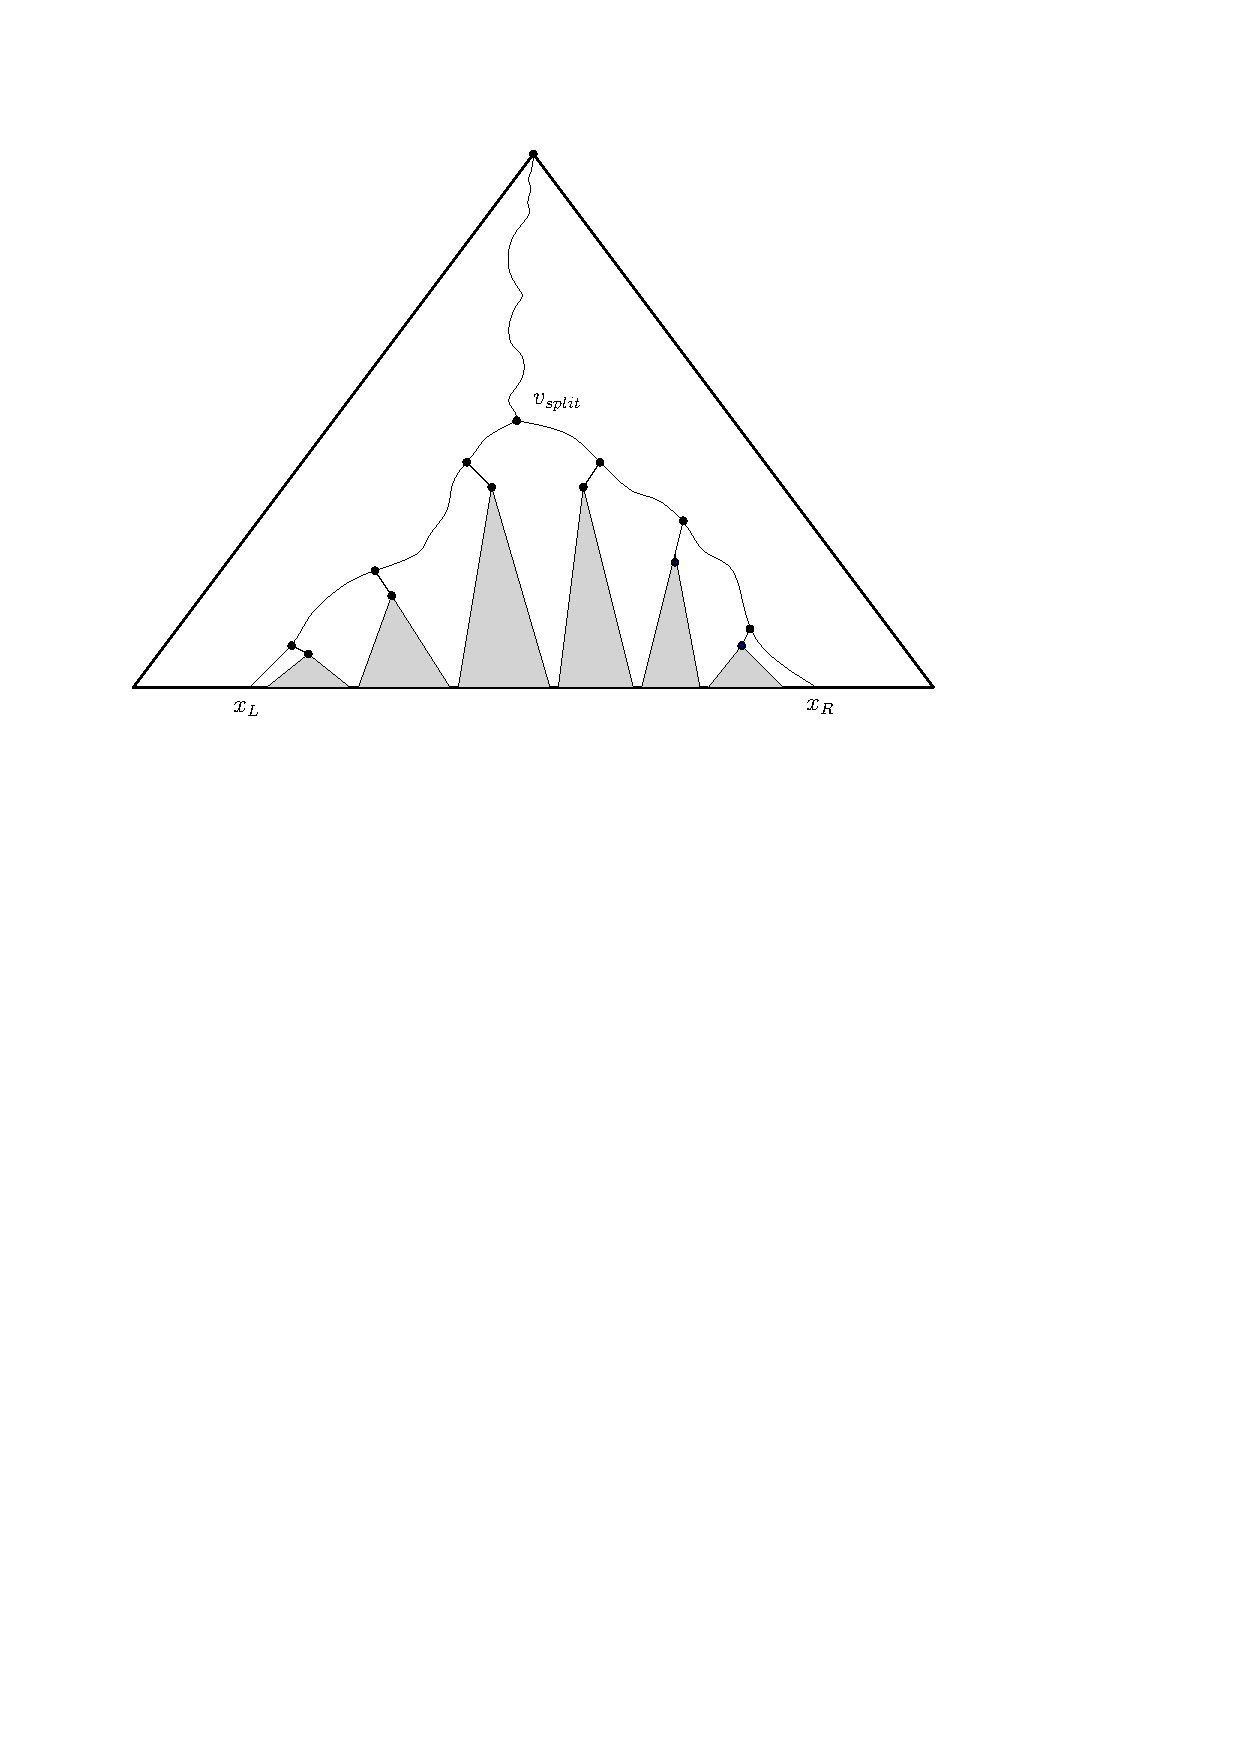
\includegraphics[scale = .5]{ipe/RQ3.pdf}
  \vspace{-0.1in}
  \caption{Querying a PST.}
  \label{fig:PST3}
\end{center}
\end{figure}

As discussed in the previous session, the running time for 2D query is of the order $T(v) = O(\log n+k)$ where $k$ denote the number of reported points. The PST for $n$ points uses $O(n \log n)$ memory space to store the data. Because along the path at each level of $x-$coordinate PST, we store each point in exactly one auxiliary PST (built on $y-$coordinate). Then, we use $O(n)$ memory space to store all nodes at each level and by considering $O(\log n)$ as the depth of $x-$coordinate PST, the total required memory would be $O(n\log n)$. In addition, the preprocessing time to build up the data structure takes $O(n \log n)$ as well. The reason is that the $y-$coordinate PST associated with each node at $x-$coordinate PST takes $O(n)$ to be constructed with bottom-up approach. Considering the fact that the depth of $x-$ coordinate PST is of the order $O(\log n)$, the total preprocessing time is bounded by $O(n\log n)$.